\documentclass[11pt]{article}
\usepackage[utf8]{inputenc}
\usepackage{textcomp}
\usepackage{listings}
\usepackage{tikz}
\usepackage{enumerate}
\PassOptionsToPackage{hyphens}{url}\usepackage{hyperref}
%\usepackage{algorithm2e}

\lstset{ %
  basicstyle=\ttfamily,commentstyle=\scriptsize\itshape,showstringspaces=false,breaklines=true,numbers=none}
\lstset{
     literate=%
         {á}{{\'a}}1
         {í}{{\'i}}1
         {é}{{\'e}}1
         {ý}{{\'y}}1
         {ú}{{\'u}}1
         {ó}{{\'o}}1
         {ě}{{\v{e}}}1
         {š}{{\v{s}}}1
         {č}{{\v{c}}}1
         {ř}{{\v{r}}}1
         {ž}{{\v{z}}}1
         {ď}{{\v{d}}}1
         {ť}{{\v{t}}}1
         {ň}{{\v{n}}}1                
         {ů}{{\r{u}}}1
         {Á}{{\'A}}1
         {Í}{{\'I}}1
         {É}{{\'E}}1
         {Ý}{{\'Y}}1
         {Ú}{{\'U}}1
         {Ó}{{\'O}}1
         {Ě}{{\v{E}}}1
         {Š}{{\v{S}}}1
         {Č}{{\v{C}}}1
         {Ř}{{\v{R}}}1
         {Ž}{{\v{Z}}}1
         {Ď}{{\v{D}}}1
         {Ť}{{\v{T}}}1
         {Ň}{{\v{N}}}1                
         {Ů}{{\r{U}}}1    
}

\newtheorem{defn}{Definition}
\newtheorem{crit}{Criterion}

\newcommand{\handout}[5]{
  \noindent
  \begin{center}
  \framebox{
    \vbox{
      \hbox to 5.78in { {\bf Intro to Methods of Software Engineering } \hfill #2 }
      \vspace{4mm}
      \hbox to 5.78in { {\Large \hfill #5  \hfill} }
      \vspace{2mm}
      \hbox to 5.78in { {\em #3 \hfill #4} }
    }
  }
  \end{center}
  \vspace*{4mm}
}

\newcommand{\lecture}[4]{\handout{#1}{#2}{#3}{#4}{Lecture #1}}
\topmargin 0pt
\advance \topmargin by -\headheight
\advance \topmargin by -\headsep
\textheight 8.9in
\oddsidemargin 0pt
\evensidemargin \oddsidemargin
\marginparwidth 0.5in
\textwidth 6.5in

\parindent 0in
\parskip 1.5ex
%\renewcommand{\baselinestretch}{1.25}

\newcommand{\squishlist}{
 \begin{list}{$\bullet$}
  { \setlength{\itemsep}{0pt}
     \setlength{\parsep}{3pt}
     \setlength{\topsep}{3pt}
     \setlength{\partopsep}{0pt}
     \setlength{\leftmargin}{1.5em}
     \setlength{\labelwidth}{1em}
     \setlength{\labelsep}{0.5em} } }
\newcommand{\squishlisttwo}{
 \begin{list}{$\bullet$}
  { \setlength{\itemsep}{0pt}
     \setlength{\parsep}{0pt}
    \setlength{\topsep}{0pt}
    \setlength{\partopsep}{0pt}
    \setlength{\leftmargin}{2em}
    \setlength{\labelwidth}{1.5em}
    \setlength{\labelsep}{0.5em} } }
\newcommand{\squishend}{
  \end{list}  }

\begin{document}

\lecture{17 --- November 20, 2018}{Fall 2018}{Patrick Lam}{version 1}

\section*{Whistleblowing}
Professional Engineers Ontario's
position is that duty-to-society absolutely exceeds duty-to-employer
with respect to ethics.

I'll reiterate that you need to check with a lawyer should you be in
a relevant situation. However, it looks like US law says that an NDA
can't restrict you from talking to the authorities. This quotation is
about securities law in particular.

\begin{quote}
Rule 21F-17, adopted pursuant to the Dodd-Frank Act, provides in relevant part:

(a) No person may take any action to impede an individual from communicating directly with the Commission staff about a possible securities law violation, including enforcing, or threatening to enforce, a confidentiality agreement … with respect to such communications\footnote{\url{https://www.lexisnexis.com/legalnewsroom/banking/b/venture-capital/archive/2015/04/15/carefully-draft-ndas-to-avoid-whistleblower-concerns.aspx}}.
\end{quote}

Ontario has similar provisions for securities law as well:

\begin{quote}
  The Anti-Confidentiality Provision provides that a provision in an agreement, including a confidentiality agreement, between a person or company and an employee of that person or company will be void to the extent that it precludes or purports to preclude the employee from whistleblowing, whether by providing applicable information to a regulatory authority, or from cooperating, testifying or otherwise assisting in an applicable proceeding (or expressing an intention to do so). It is important to note that, while the Anti-Confidentiality Provision voids a confidentiality provision to the extent it prevents disclosure, the approach in the U.S. is somewhat different, as in the U.S. it is a breach of securities law to impede disclosure (including through the use of overly broad confidentiality language)\footnote{\url{https://www.osler.com/en/resources/regulations/2016/a-review-of-new-whistleblower-protections-under-on}}.
\end{quote}

This is via an updated Ontario Securities Law as of this past July. This applies to securities law, but a whole lot of things\footnote{Matt Levine of Bloomberg writes ``Everything is securities fraud!''} are covered under securities law. 
\newpage
\section*{Licensing}
To practice professional engineering in Canada, you must have a license (PEng).

\begin{quote}
The practice of professional engineering is defined in Section 1 of the Professional Engineers Act and comprises of three tests. Professional engineering is:

\begin{enumerate}
\item    any act of planning, designing, composing, evaluating, advising, reporting, directing or supervising (or the managing of any such act);
\item    that requires the application of engineering principles; and
\item    concerns the safeguarding of life, health, property, economic interests, the public welfare or the environment, or the managing of any such act.
\end{enumerate}

\hfill \url{http://peo.on.ca/index.php?ci_id=1813&la_id=1}
\end{quote}

To get a PEng in Ontario, you need to:
\begin{enumerate}
\item have an accredited engineering degree (e.g. the BSE);
\item pass the Professional Practice Exam (law and ethics);
\item practice for 4 years, which must include 12 months in Canada under the supervision of a Professional Engineer, and which may include 12 months before graduation after 2B.
\end{enumerate}

\section*{Standards}

\begin{center}
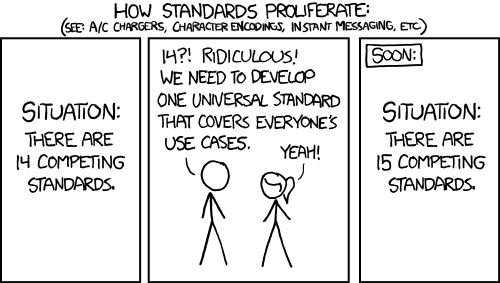
\includegraphics[width=.7\textwidth]{images/L17-standards.png}\\
\url{https://xkcd.com/927/}
\end{center}

We couldn't exist in society without standards. Life before USB was terrible, but even then, there were standard serial and parallel ports. But how could you even plug in your devices to the wall? And, at a higher level, how do you get information from the Internet?

Standards can be ambiguous and implementations can be outright wrong. The robustness principle, also known as Postel's Law\footnote{Jon Postel. \emph{Transmission Control Protocol.} IETF. RFC 761.}, was key to the early Internet working at all.
\begin{quote}
  Be conservative in what you do,\\
  be liberal in what you accept from others.
\end{quote}

Unfortunately, there are pitfalls to implementing Postel's Law. An alternate view is ``systems should fail spectacularly and destructively''. Discuss.

\section*{The Environment}
We talked about this to some extent previously in the context of Volkswagen, but you could blame the automotive engineers for that. Let's talk about it more directly with respect to software.

\noindent
Reference: San Murugesan, ``Harnessing Green IT: Principles and Practices.'' IEEE \emph{IT Professional}, January--February 2008, pp. 24--33.

Environmental impacts of computing:
\begin{itemize}
\item manufacturing the computers;
\item operating the computers: power (from which source?) and cooling (especially in data centres);
\item decommissioning them.
\end{itemize}

Some possible mitigations:
\begin{itemize}
\item use fewer computers, e.g. via virtualization;
\item deploy computers where they need less cooling (e.g. Iceland);
\item power off/suspend computers when not in use;
\item put fewer harmful substances (e.g. lead) in them; recycle these substances.
\end{itemize}

In this week's assignment I ask you to estimate the payroll costs of waiting for systems to come online versus the electricity costs for those systems.



%regulations, standards, the environment

\end{document}

